\documentclass[a4paper]{article}



\usepackage{Sweave}
\begin{document}
\Sconcordance{concordance:example2.tex:example2.rnw:%
1 4 1 1 0 4 1 1 2 4 0 1 2 1 1 1 2 1 0 1 1 3 0 1 2 3 1 1 -6 1 0 1 1 1 8 %
1 1 19 0 1 1 4 0 1 2 2 1}



First we define a figure hook:
\begin{Schunk}
\begin{Sinput}
> options(SweaveHooks = list(fig = function() par(mfrow=c(2,2))))
\end{Sinput}
\end{Schunk}

Then we setup variable definitions without actually evaluating them
\begin{Schunk}
\begin{Sinput}
> x <- 1:10
> y <- rnorm(x)
\end{Sinput}
\end{Schunk}


Then we put the pieces together:
\begin{center}
\begin{Schunk}
\begin{Sinput}
> x <- 1:10
> y <- rnorm(x)
> lm1 <- lm(y~x)
> summary(lm1)
\end{Sinput}
\begin{Soutput}
Call:
lm(formula = y ~ x)

Residuals:
    Min      1Q  Median      3Q     Max 
-1.1293 -0.5027 -0.0845  0.4978  1.5294 

Coefficients:
            Estimate Std. Error t value Pr(>|t|)
(Intercept)  0.65213    0.62267   1.047    0.326
x           -0.05581    0.10035  -0.556    0.593

Residual standard error: 0.9115 on 8 degrees of freedom
Multiple R-squared: 0.03723,	Adjusted R-squared: -0.08312 
F-statistic: 0.3093 on 1 and 8 DF,  p-value: 0.5933 
\end{Soutput}
\begin{Sinput}
> plot(lm1)
\end{Sinput}
\end{Schunk}
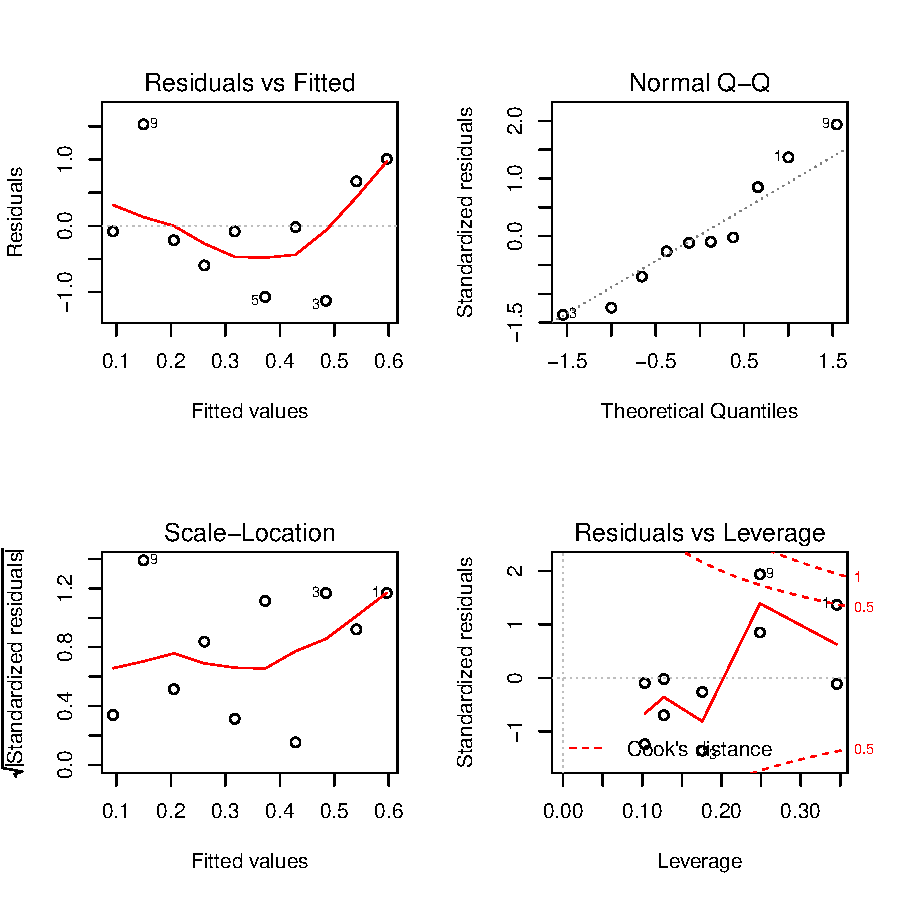
\includegraphics{example2-003}
\end{center}

\end{document}
